\section{Results}
\label{sec:result}
To test the performance of RMW between 1 to 10,000,000 bytes are generated in different test cases.
PMW is implemented in C++ and uses the standard library of C++ along with Boost C++ Libraries~\citep{boost}.
The test cases are run on an Intel Core i7 2.93 GHz with 8 GB RAM operated by Windows 7 64 bit SP 1.

The results of the performance tests are shown in Table~\ref{tab:tests}
For comparison the standard library random number generator in C has a throughput of $\approx 7500$ samples/ms and \devrandom{} has a throughput $<0.001$ sample/ms $=1$ sample/s.
Note that \devrandom{} is run on another computer running Ubuntu OS, with an initially empty pool of entropy.
This computer is a server and hence has no directly connected keyboard or mouse.

\begin{figure}[hbt]
	\centering
		\begin{tabular}{|l|l|l|}
			\hline
			Samples&Time (ms)&Throughput (samples/ms)\\
			\hline
			1&5&0.20\\
			\hline
			10&18&0.56\\
			\hline
			100&38&2.6\\
			\hline
			1,000&90&11\\
			\hline
			10,000&740&14\\
			\hline
			100,000&7202&14\\
			\hline
			1,000,000&83314&12\\
			\hline
			10,000,000&853632&12\\
			\hline
		\end{tabular}
	\caption{Results from performance tests}
	\label{tab:tests}
\end{figure}

In combination with the performance tests the generated numbers are logged and a distribution can be seen in Figure~\ref{fig:distribution}.
The bytes are represented by their decimal values.
The figure shows the number of occurrences of each byte value (0-255 in decimal).
A mean line is shown in red.

\begin{figure}[hbt]
	\centering
		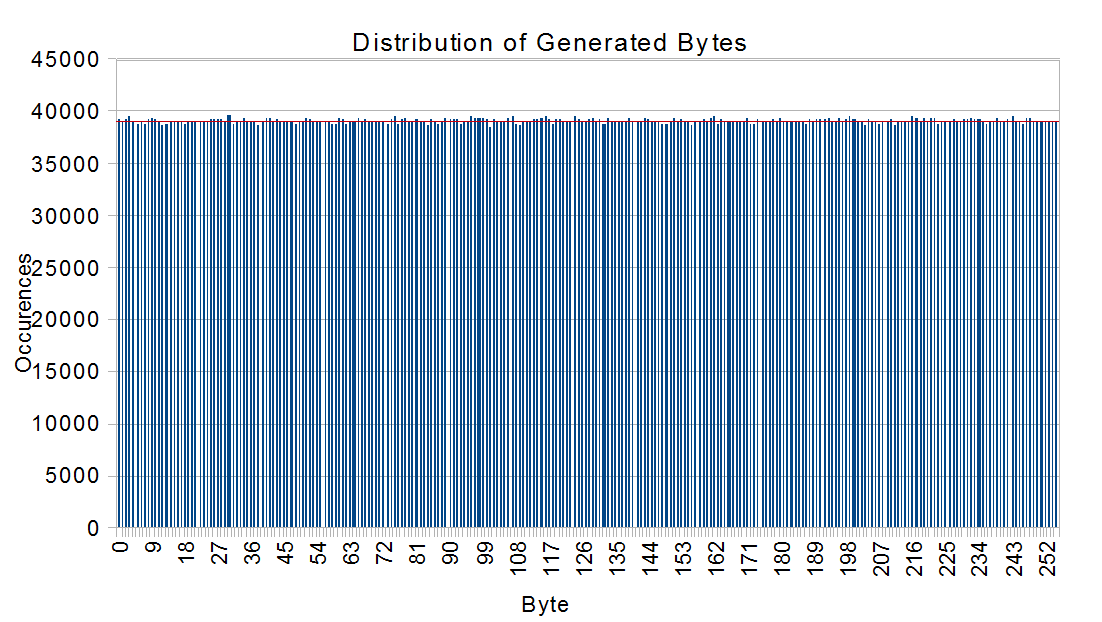
\includegraphics[width=\columnwidth]{image/distribution.png}
	\caption{Distribution of $10^7$ random bytes.}
	\label{fig:distribution}
\end{figure}
